We set up our optimization with two different turbine groups. We assigned each turbine to one of two groups, where all turbines in a group had the same tower hub height, rotor diameter, turbine rating, tower diameter, and tower shell thickness.
% Manufacturing each tower with custom dimensions may be very expensive, and further study will be necessary to determine if it is worth the additional cost and complexity to design each turbine individually. 
Rather than optimize each turbine, we chose two groups because our previous study in which we optimized wind farms with different turbine heights indicated that the most benefit comes from increasing from one height group to two. Any benefit from introducing more groups was marginal \citep{stanley2018}. We parameterized the tower by specifying the diameter and shell thickness at the bottom, midpoint, and top of the tower and then linearly interpolating diameter and shell thickness at points in between. 
        
        It may be beneficial to do a binary optimization in which each turbine can change the turbine group to which it belongs, but this greatly increases the complexity of the optimization and makes it gradient-free. Binary variables, such as turbine group assignment, have no intermediate values. They are either one or the other. This means there is no way to use gradients in their optimization. Gradient-free optimization is more computationally expensive, which severely limits the number of design variables we can include in the problem. To maintain the gradient-based optimization, we assigned each turbine to one of the groups before starting the optimization. Once assigned a turbine could not switch to the other group. In this study, we only examine an equal weighting of turbines in each group, but additional benefit may come from optimally choosing the number of turbines in each group.% However, we did explore the effect of including different ratios of the different turbine groups, including 1-1, 2-1, and 3-1.
        
        We ran several cases in which different design variables were included in the problem to allow comparison of their effects on COE. In all, the design variables we included were the position of each turbine ($x_i,y_i$), the tower height of each group ($H_1, H_2$), the rotor diameter of each group ($D_1, D_2$), the rated power of each group ($R_1, R_2$), the tower diameter of each group ($d_{1,j}, d_{2,j}$), and the tower shell thickness of each group ($t_{1,j}, t_{2,j}$). Index j refers location on the tower (j=1 is at the bottom, j=2 at the midpoint, j=3 at the top), meaning there are six total variables to define diameter (three for each height group), and six to define the tower shell thickness.
                
             
          The turbine layout and structural constraints are that were previously formulated in our multiple-hub-height study \citep{stanley2018}. Because rotor diameter was a design variable, the turbine spacing constraint was slightly reformulated such that the distance between any two turbines in the wind farm was greater than the sum of the two rotor diameters.
           The rotor diameter and the turbine rating were constrained by the lowest and highest values that were included in the RotorSE optimization. This constraint is defined from the upper and lower functioning limits of RotorSE. The lower limits were never active in these optimizations, however some of the upper limits were active as will be seen in the Results section.
       The optimization can be expressed:
        
        
        \begin{equation}
			\begin{aligned}
				& \text{minimize}
					& & \text{COE} \\
                & \text{w.r.t.} 
                	&& x_i,~ y_i,~ H_{1,2},~ D_{1,2},~ R_{1,2},~ d_{(1,j)},~ d_{(2,j)},~ t_{(1,j)},~t_{(2,j)}\\
                		&&& i = 1, \ldots, n; \; j = 1,~2,~3 \\
				& \text{subject to}
% 					& & x_{\text{initial, min}} \leq x_i \leq x_{\text{initial, max}} \\
					& & \text{boundary constraints} \\
%                         &&& y_{\text{initial, min}} \leq y_i \leq y_{\text{initial, max}} \\
						&&& \sqrt{(x-x_i)^2+(y-y_i)^2} \geq 2D_{\text{rotor}} \\
						&&& H_1-\frac{D_1}{2}, H_2-\frac{D_2}{2} \geq 10~ \text{m}\\
                		&&& d_{(1,j),(2,j)} \leq 6.3~ \text{m}\\
                		&&& d_{(1,top),(2,top)} \geq 3.87~ \text{m}\\
						&&& \frac{3\hspace{0.08cm}\Omega}{1.1} \geq f_{1,2} \geq 1.1\hspace{0.08cm}\Omega \\
                		&&& \text{shell buckling margins: max thrust} \leq 1 \\
                        &&& \text{shell buckling margins: survival load} \leq 1 \\
                		&&& \frac{d_{(1,j)}}{t_{(1,j)}},\frac{d_{(2,j)}}{t_{(2,j)}} \geq 120\\
                        &&& 46~ \text{m} < D_1,D_2 < 160~ \text{m}  \\
                        &&& 500~ \text{kW} < R_1,R_2 < 10,000~ \text{kW} \\
			\end{aligned}
		\end{equation}
%
Note that i is the index defining the wind turbine, and j is the index describing the location on the tower.
        
        The gradients for this optimization were all analytic. We calculated the partial derivatives of each small section of the model and included each part in a framework called OpenMDAO, which calculates the gradients of the entire system \citep{gray2010openmdao}. The analytic gradients are significant because they are more accurate, converge to better solutions, and converge on the solution much faster that finite difference gradients. More importantly, they allow us to solve much larger optimization problems. % These analytic gradients allow coupled optimization of turbine position, height, diameter and thickness, and yaw in each wind direction. Including yaw introduces thousands of design variables, and is nearly impossible to optimize with gradient-free methods and very time-consuming with finite difference gradients.  
        
We optimized two different wind farms, each with several different wind shear exponents and turbine spacing multipliers as will be explained later in this section. 
The first wind farm is a fictional 32-turbine wind farm with a circular boundary. %The baseline layout and boundary is shown in Fig. \ref{circular_layout}. 
This wind farm was optimized with wind data from the city of Alturas, California, shown in Fig. \ref{wind_roses}.  For lack of reliable data, the average wind speed from each direction of this wind rose was assumed to eight meters per second, shown in Fig \ref{wind_speeds}.
The second wind farm is the Princess Amalia wind farm, a real farm off the coast of the Netherlands, which has 60 wind turbines. This wind farm was optimized with the wind direction and average directional speed data from the true Princess Amalia farm, shown in Figs. \ref{wind_roses} and \ref{wind_speeds}. The farm boundary for the Princess Amalia wind farm is the convex hull of the original Princess Amalia layout. The baseline turbine layout and boundaries are shown in Fig. \ref{layouts}. The turbines in both wind farms are Vestas 2 Megawatt wind turbines, which have a rotor diameter of 80 meters. Therefore, we used a baseline rotor diameter of 80 meters and a baseline power rating of 2 Megawatts. The baseline hub height used in this study was 100 meters. 

\begin{figure}[htbp]
  \centering
  %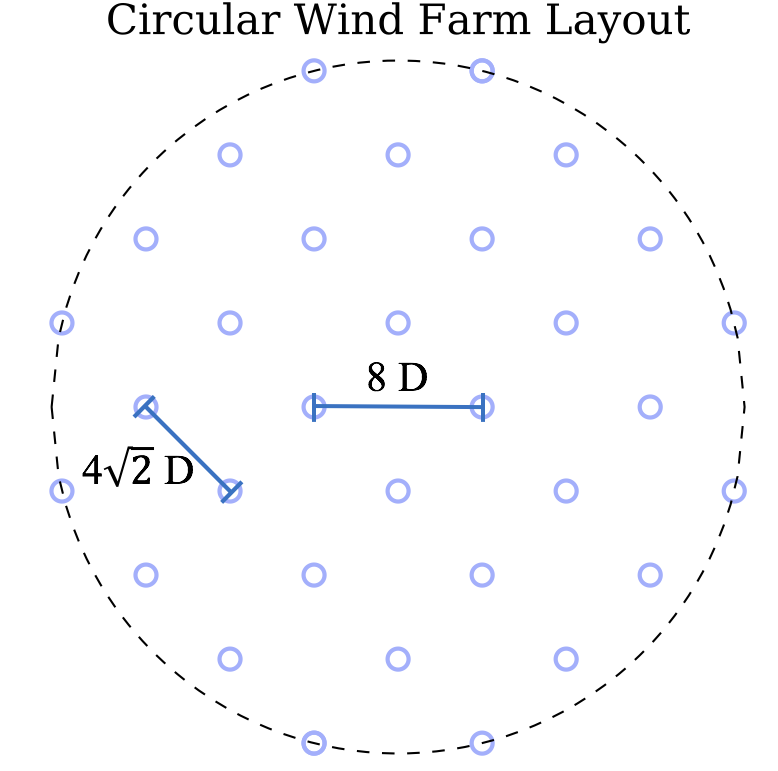
\includegraphics[trim={1cm 0 0 0},clip,width=0.4\textwidth]{Figures/circular.png}
  %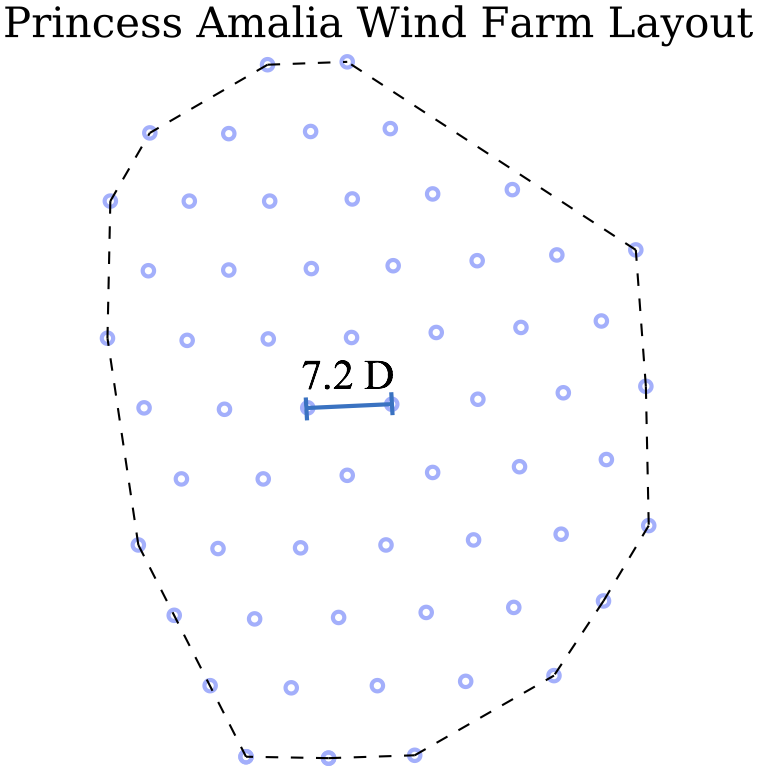
\includegraphics[trim={0 0 1cm 0},width=0.392\textwidth]{Figures/amalia.png}
   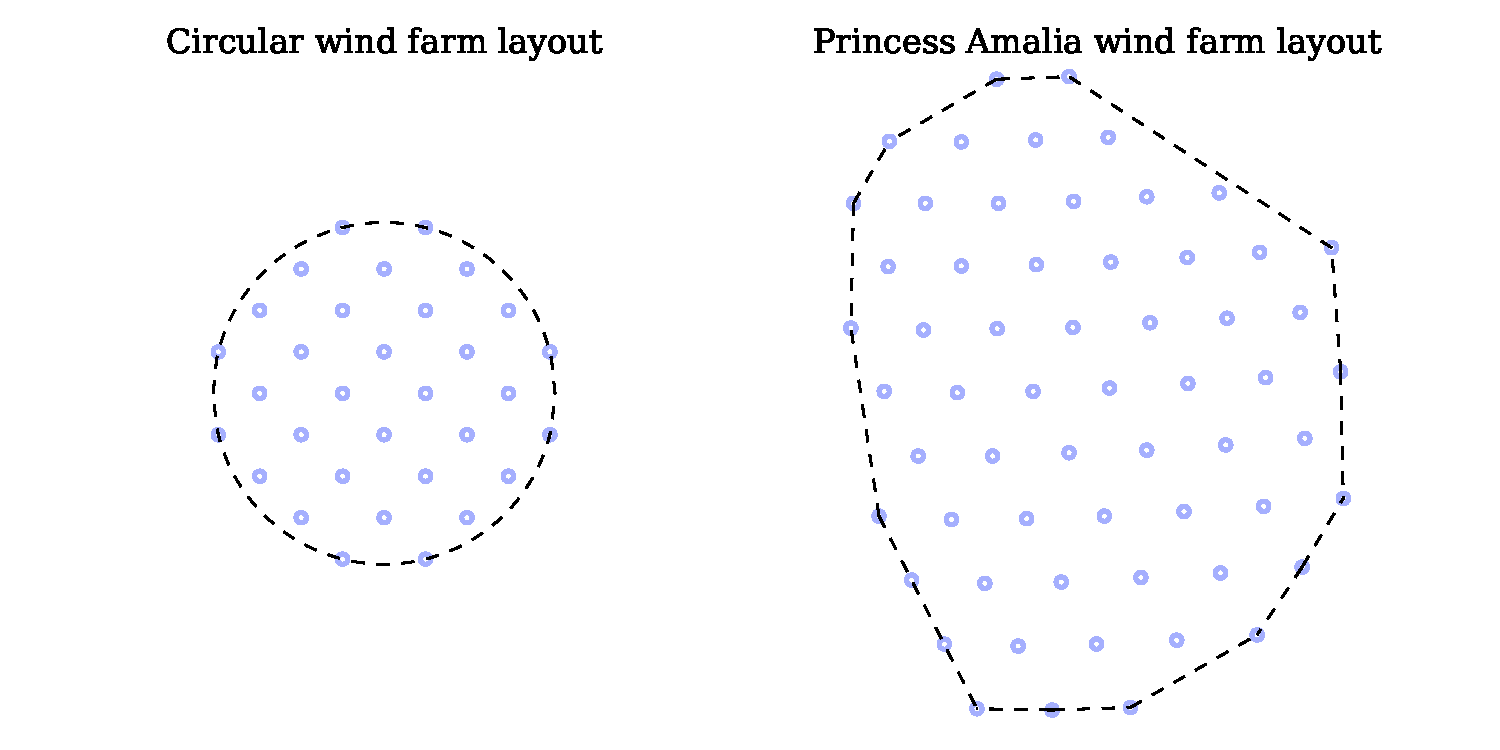
\includegraphics[width=0.7\textwidth]{Figures/baseline_layouts.pdf}
  \caption{\label{layouts} The two different wind farm designs that were optimized. On the left is a contrived circular wind farm design with 32 turbines. On the right is the Princess Amalia wind farm, an offset grid design with 60 wind turbines. }
\end{figure}

\begin{figure}[htbp]
  \centering
  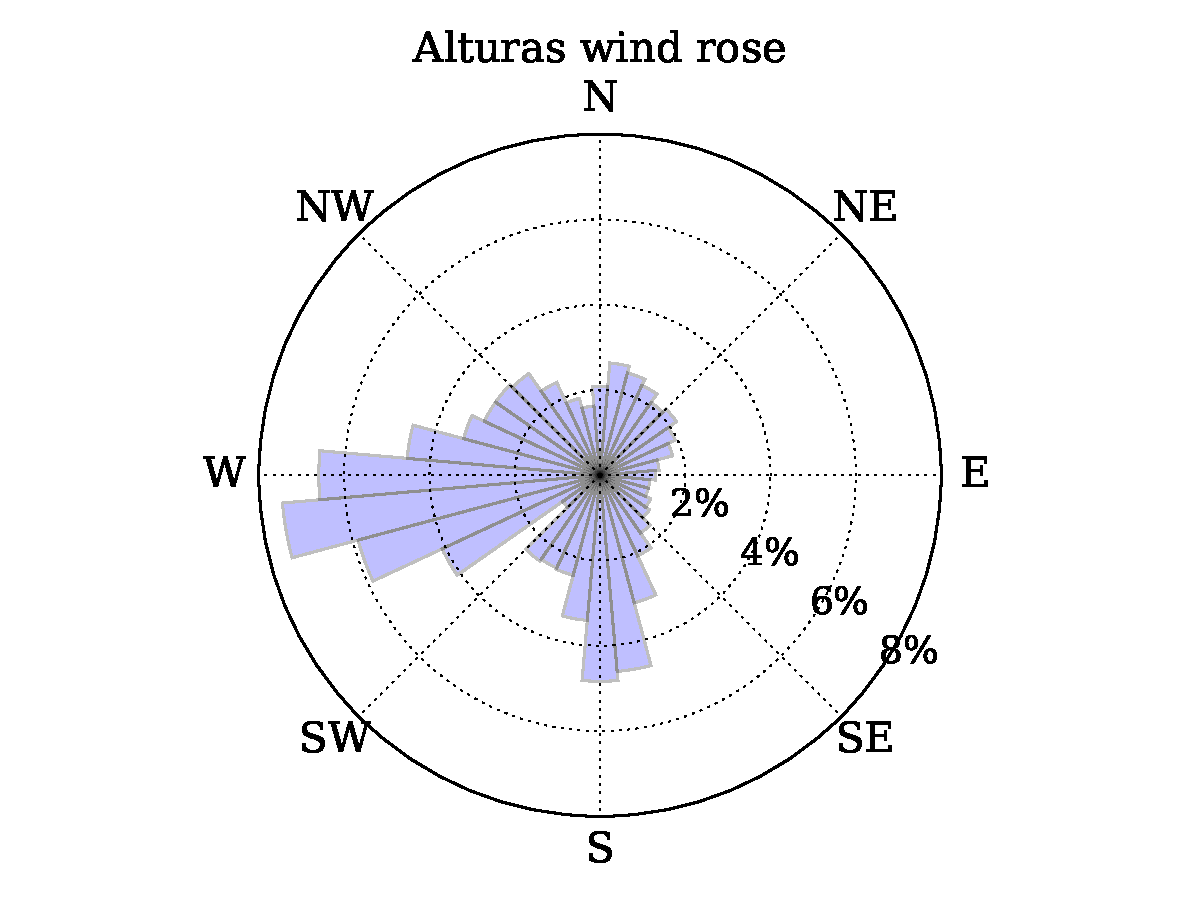
\includegraphics[width=0.49\textwidth]{Figures/alturas_rose.pdf}
  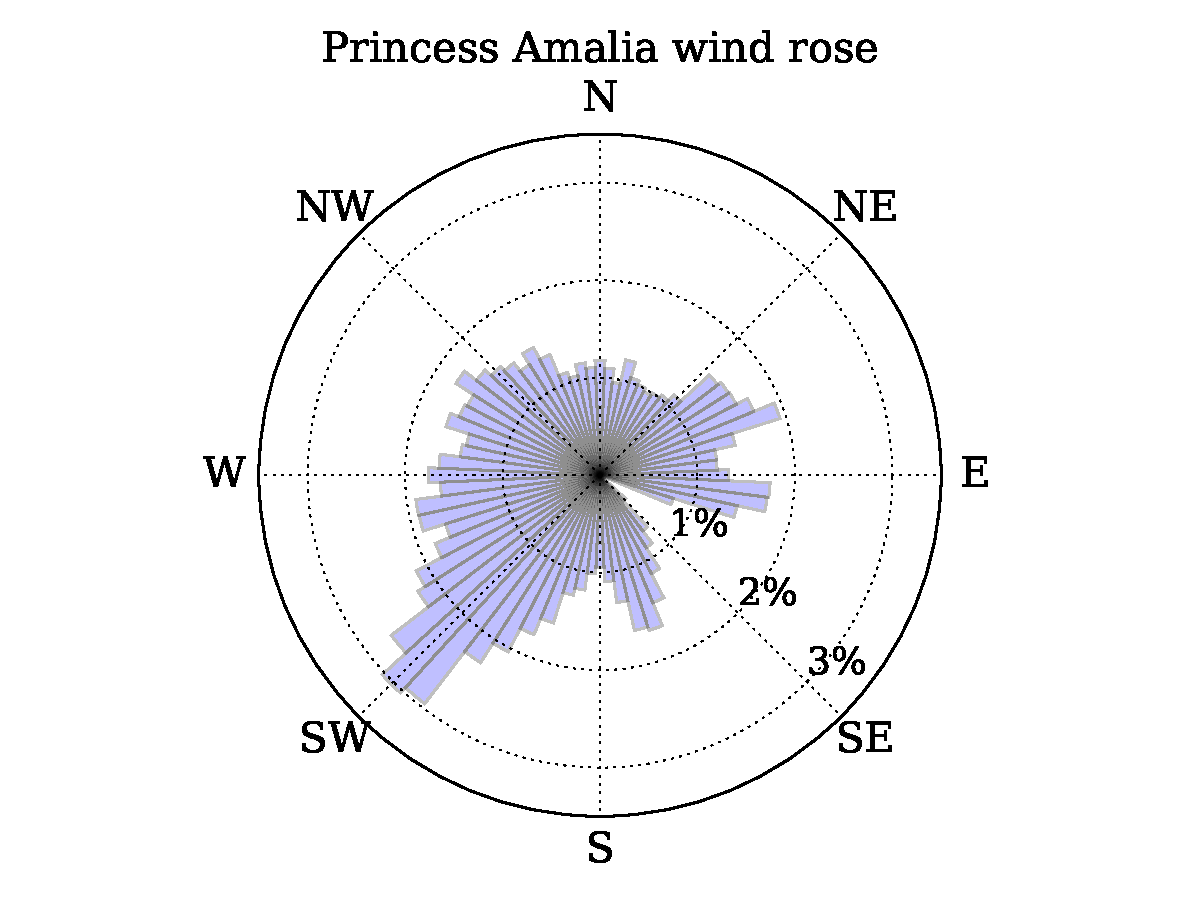
\includegraphics[width=0.49\textwidth]{Figures/amalia_rose.pdf}
  \caption{\label{wind_roses} On the left, the wind direction distribution in Alturas, California, separated into 36 bins, every 10 degrees. On the right, the wind direction distribution of the Princess Amalia Wind Farm, separated into 72 bins, every 5 degrees.}
\end{figure}

\begin{figure}[htbp]
  \centering
  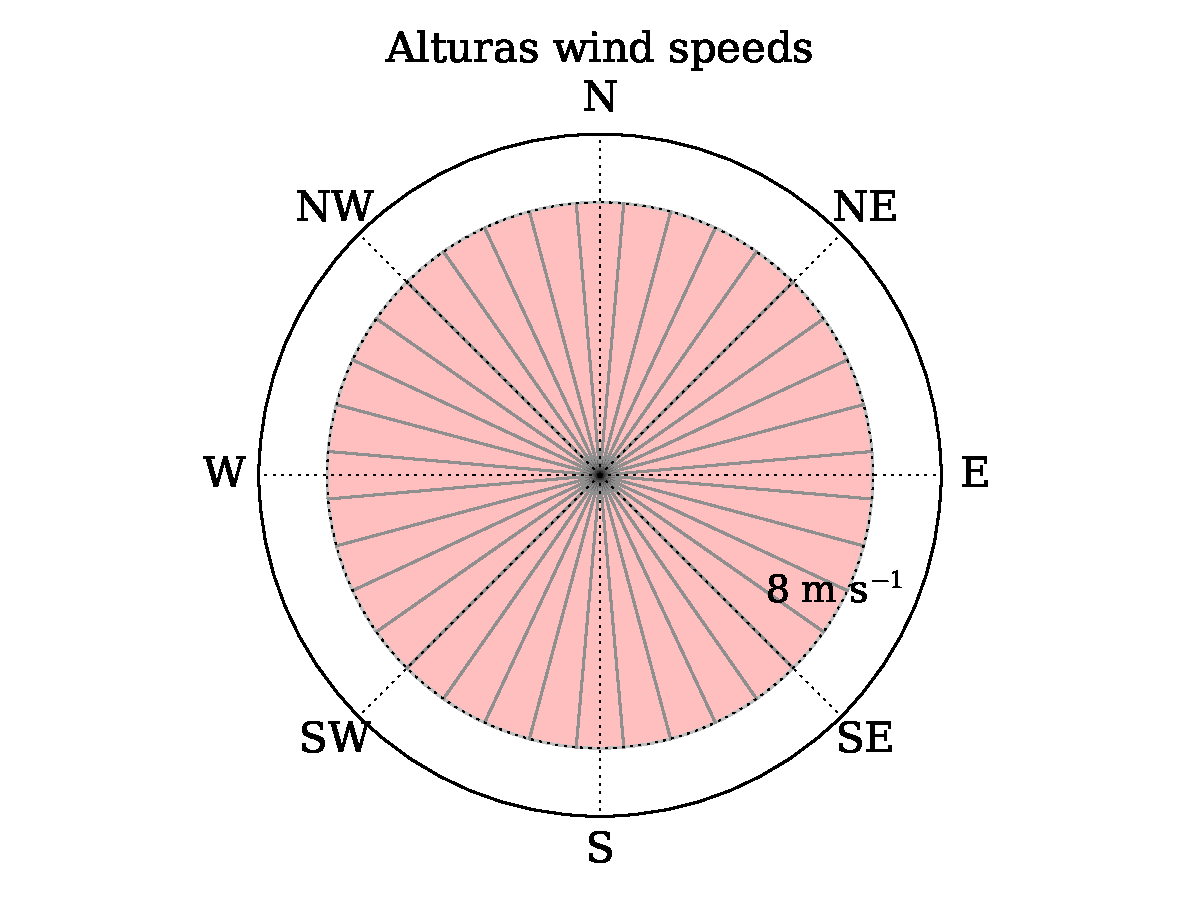
\includegraphics[width=0.49\textwidth]{Figures/alturas_speeds.pdf}
  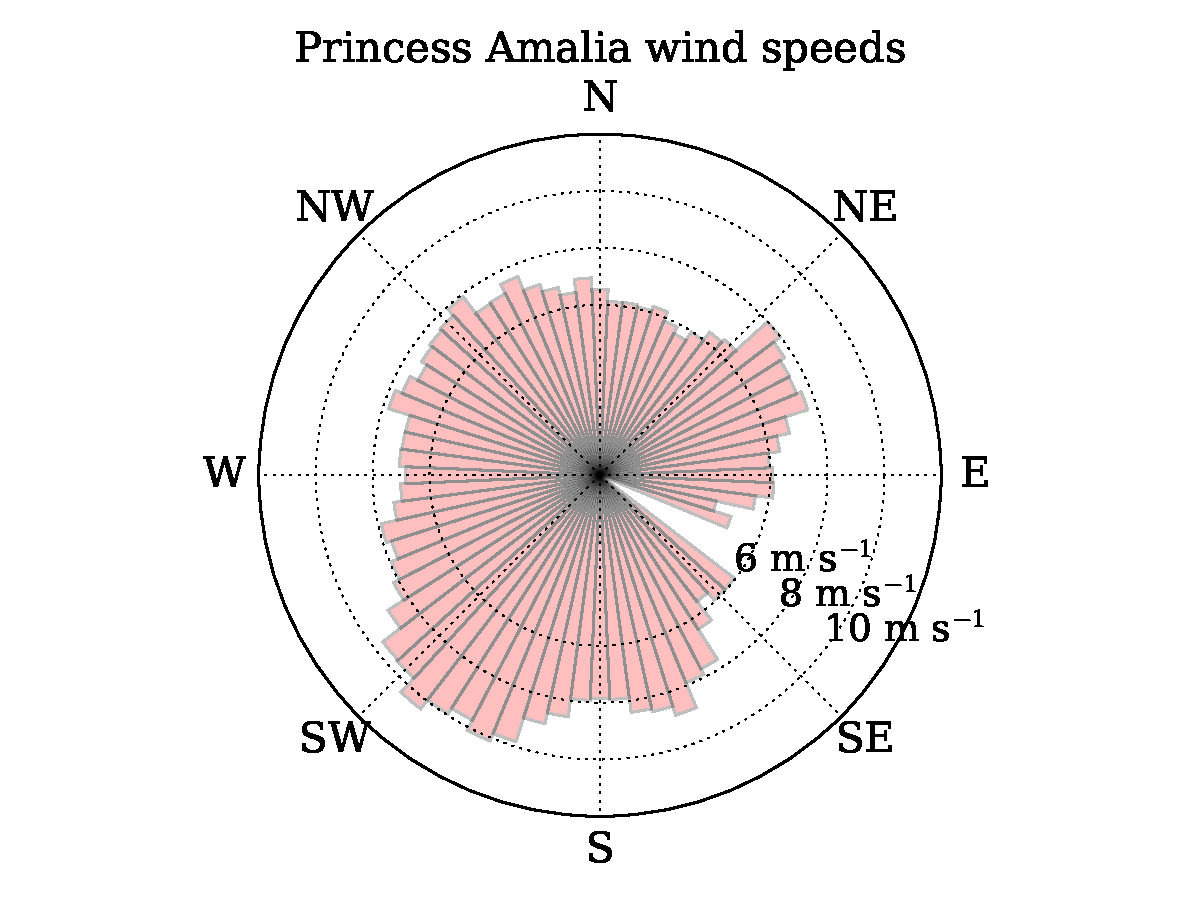
\includegraphics[width=0.49\textwidth]{Figures/amalia_speeds.pdf}
  \caption{\label{wind_speeds} On the left, the assumed directionally averaged wind speeds for Alturas, California, separated into 36 bins, every 10 degrees. Each direction is assumed to have an average wind speed of 8 meters per second. On the right, the directionally averaged wind speeds of the Princess Amalia Wind Farm, separated into 72 bins, every 5 degrees.}
\end{figure}


We optimized each of the wind farms shown in Fig. \ref{layouts} with three different wind shear exponents (0.075, 0.175, 0.275), and three different spacing multipliers (0.5, 1.0, 1.5). The wind shear exponent defines how fast the wind speed changes with height, as seen in Equation \ref{Eq:shear}. Low shear exponents are typical over open water or flat plains, while higher shear exponents exist in areas with a lot of large trees or buildings. Figure \ref{shear_profile} shows the wind speed profiles of the three shear exponents we used. For a shear exponent of 0.075, there is only an 8.6\% increase in the wind speed from the reference height of 50 meters to 150 meters. For a shear exponent of 0.175 there is a wind speed increase of 21.2\% for the same height difference, and for a shear exponent of 0.275 the wind speed increase is 35.3\% from 50 to 150 meters. We also optimized each wind farm for different turbine spacings by adjusting the turbine locations by some spacing multiplier, $\beta$.  This is simply some constant multiplied to each turbine location. The wind farm boundaries were adjusted accordingly with the spacing multipliers, meaning for radius of the circular wind farm was also multiplied by the spacing multiplier, and the convex hull of the Princess Amalia farm was applied to the adjusted turbine locations. Figure \ref{farm_spacings} shows both of the wind farms adjusted by the spacing multipliers, as well as the turbine spacing in baseline rotor diameters. As the turbine designs are optimized, these spacings (in rotor diameters) will increase or decrease according. Note that in the circular wind farm, the turbine distances are presented in the rows closely inline with the dominant wind direction. The closest neighboring turbines are actually $\sqrt{2}/2$ multiplied by this value. 


\begin{figure}[htbp]
  \centering
  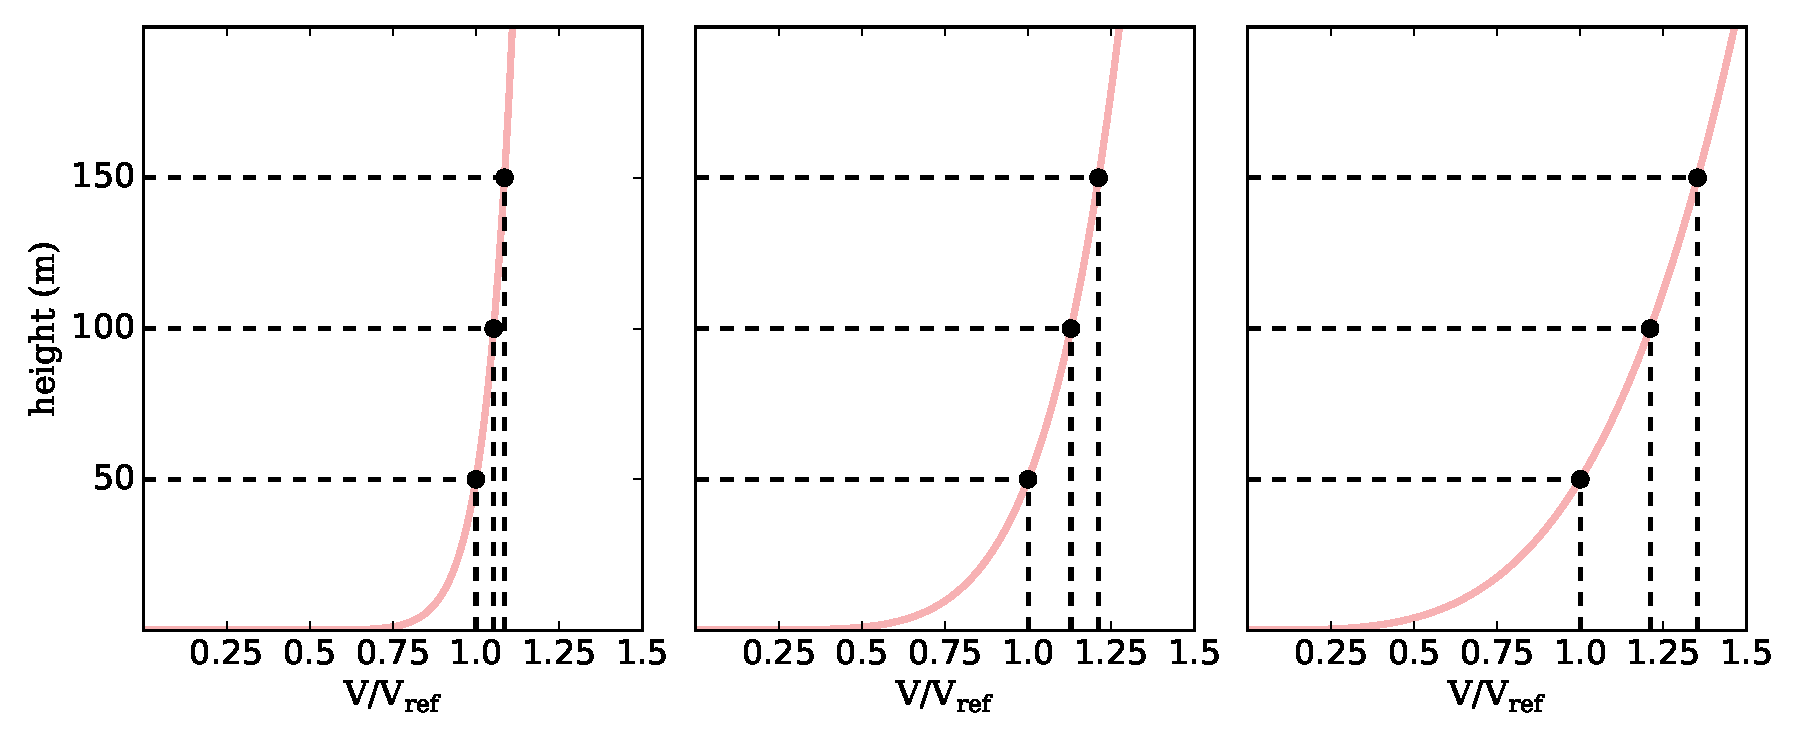
\includegraphics[width=0.7\textwidth]{Figures/shears.pdf}
  %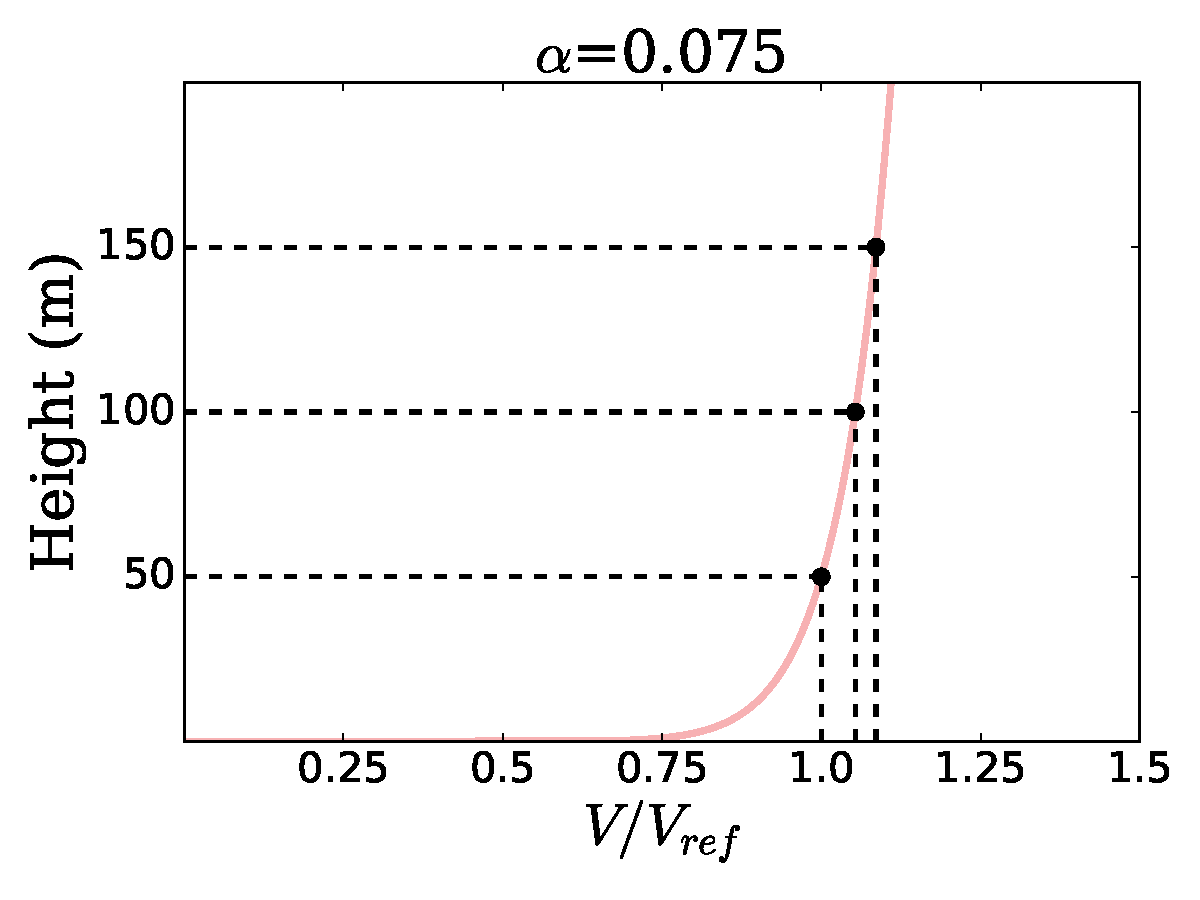
\includegraphics[width=0.49\textwidth]{Figures/windProfile_0_075.pdf}
  %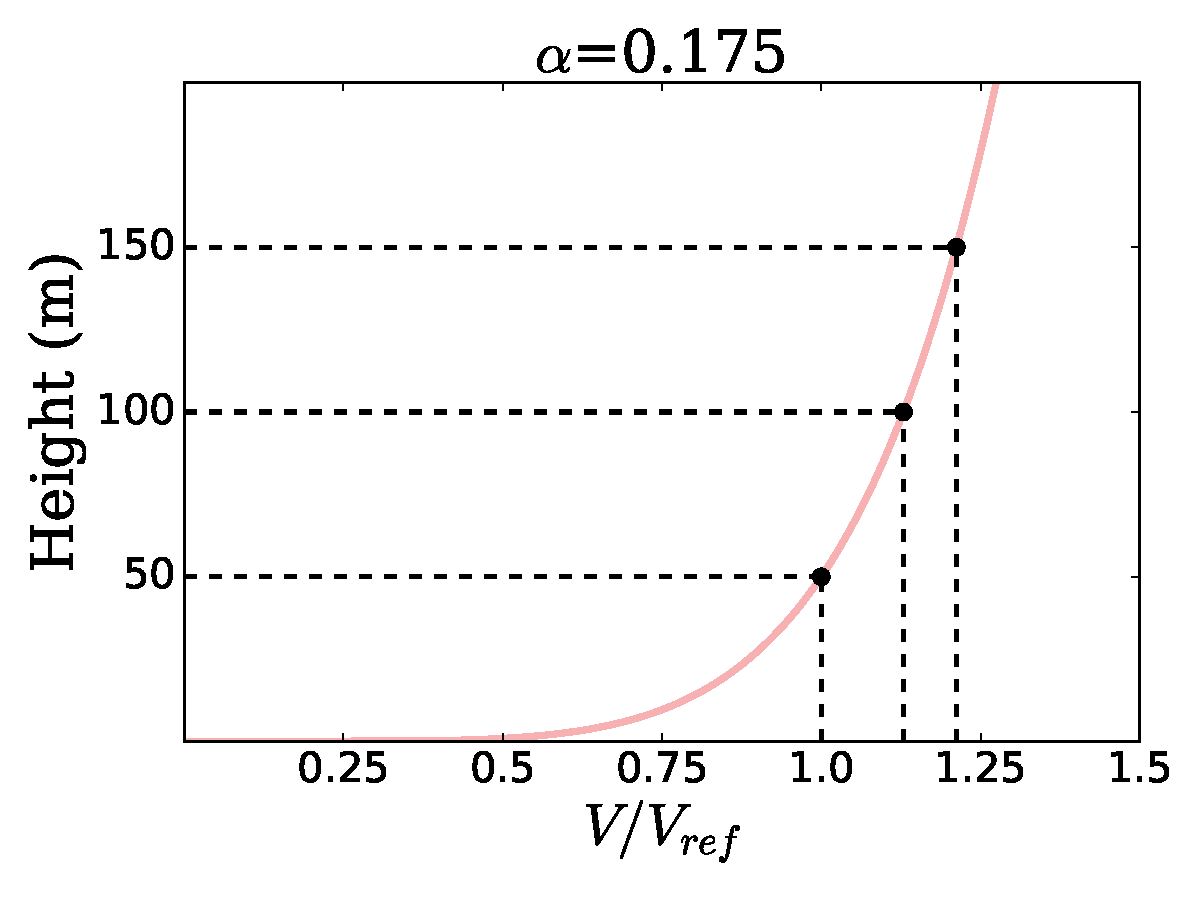
\includegraphics[width=0.49\textwidth]{Figures/windProfile_0_175.pdf}
  %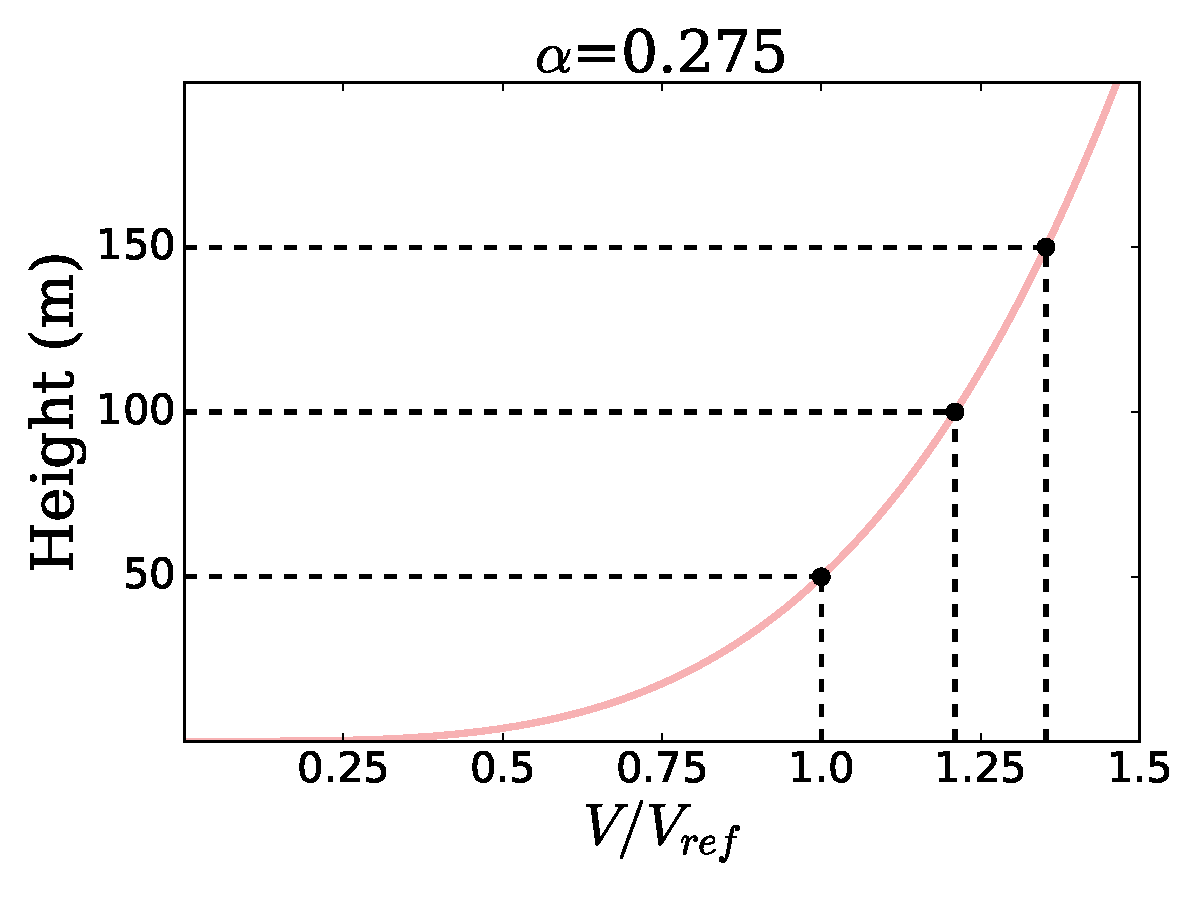
\includegraphics[width=0.49\textwidth]{Figures/windProfile_0_275.pdf}
  \caption{\label{shear_profile}The wind speed profiles for various wind shear exponents. With lower shear exponents, like $\alpha=0.075$ shown in Fig. \ref{wp075}, the wind speed does not vary dramatically with height. For higher wind shear, like $\alpha=0.275$ shown in Fig. \ref{wp275}, there is a significant wind speed increase with height.}
\end{figure}

\begin{figure}[htbp]
  \centering
  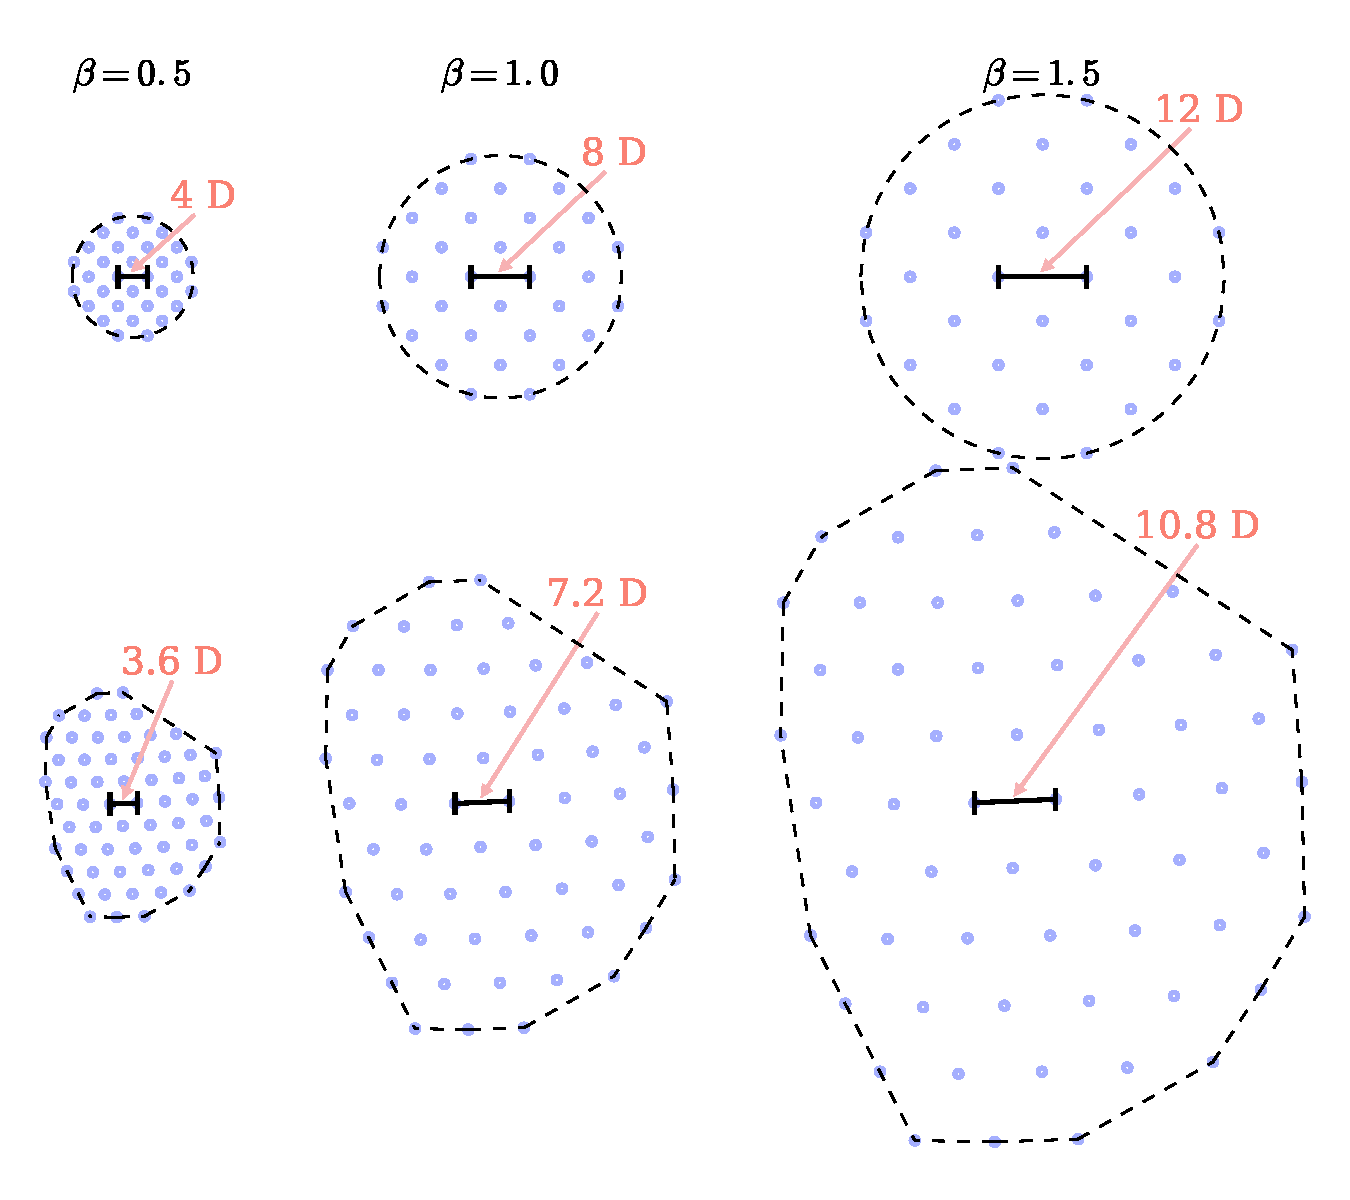
\includegraphics[width=0.7\textwidth]{Figures/spacing_multipliers.pdf}
  %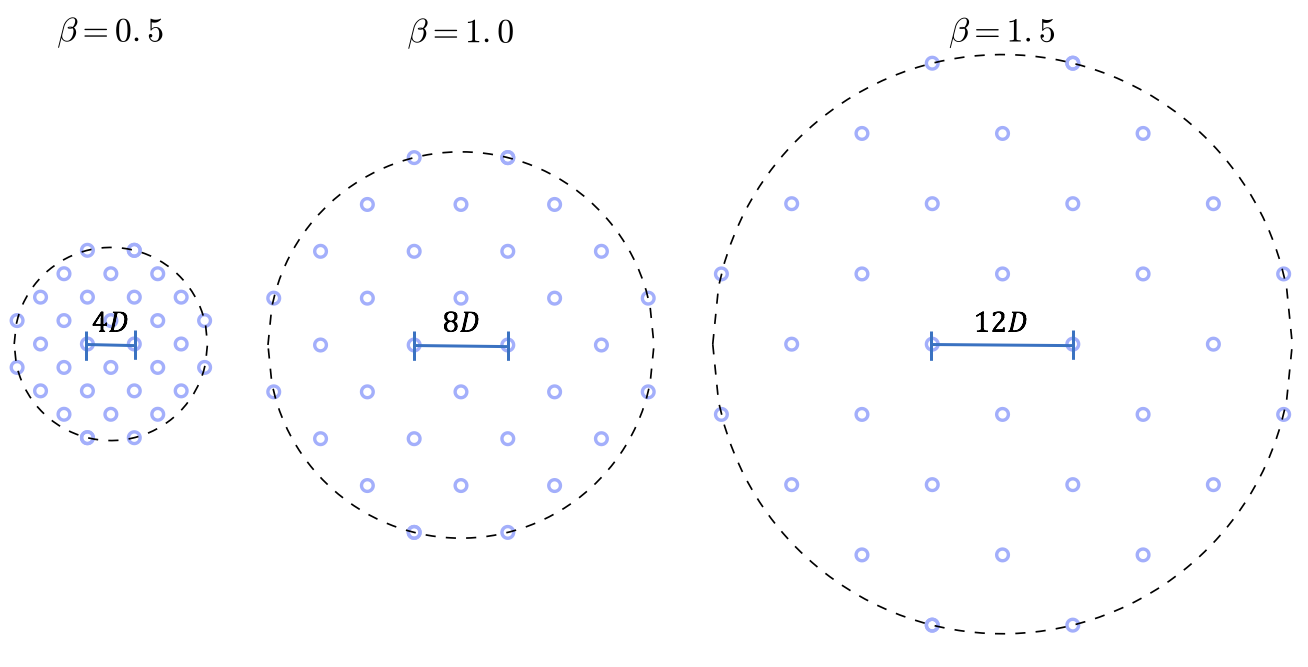
\includegraphics[width=\textwidth]{Figures/circle_spacings.png}
  %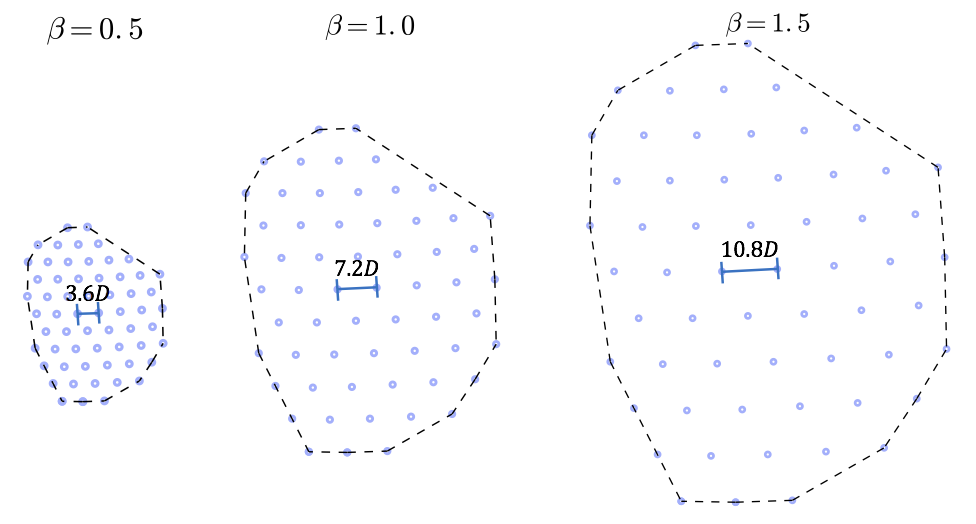
\includegraphics[width=.88\textwidth]{Figures/amalia_spacings.png}
  \caption{\label{farm_spacings}The six wind farm boundaries and associated baseline layouts optimized in this study. The same two layouts were multiplied by a spacing multiplier, $\beta=0.5,1.0,1.5$, which changed the wind farm size and the averaging spacing between wind turbines.  On the top is the 32-turbine, circular wind farm, and on the bottom is the 60-turbine, Princess Amalia wind farm. The turbine spacings, in baseline rotor diameters, are also displayed for each spacing multiplier in this figure.}
\end{figure}

The results of gradient-based optimization, especially for problems with many local minima, are sensitive to the starting location. As in most optimization problems, there is no guarantee that the solution is the global solution. The best results can be achieved with a multiple-start approach, where several different starting points are used for each condition, and the best solution is used. In our study, we started each turbine location from the Princess Amalia or circular wind farm baseline locations in Fig. \ref{farm_spacings}, each perturbed by a random amount. All of the other design variables were initialized randomly.

% \begin{figure}[htbp]
%   \centering
%   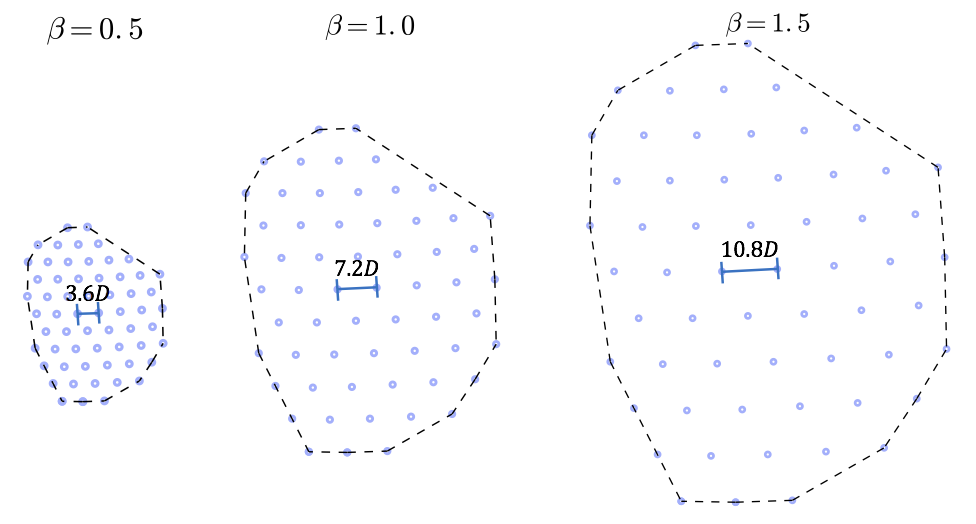
\includegraphics[width=\textwidth]{Figures/amalia_spacings.png}
%   \caption{\label{amalia_spacings} \textbf{CAPTION HERE}}
% \end{figure}

% \begin{figure}[htbp]
%   \centering
%   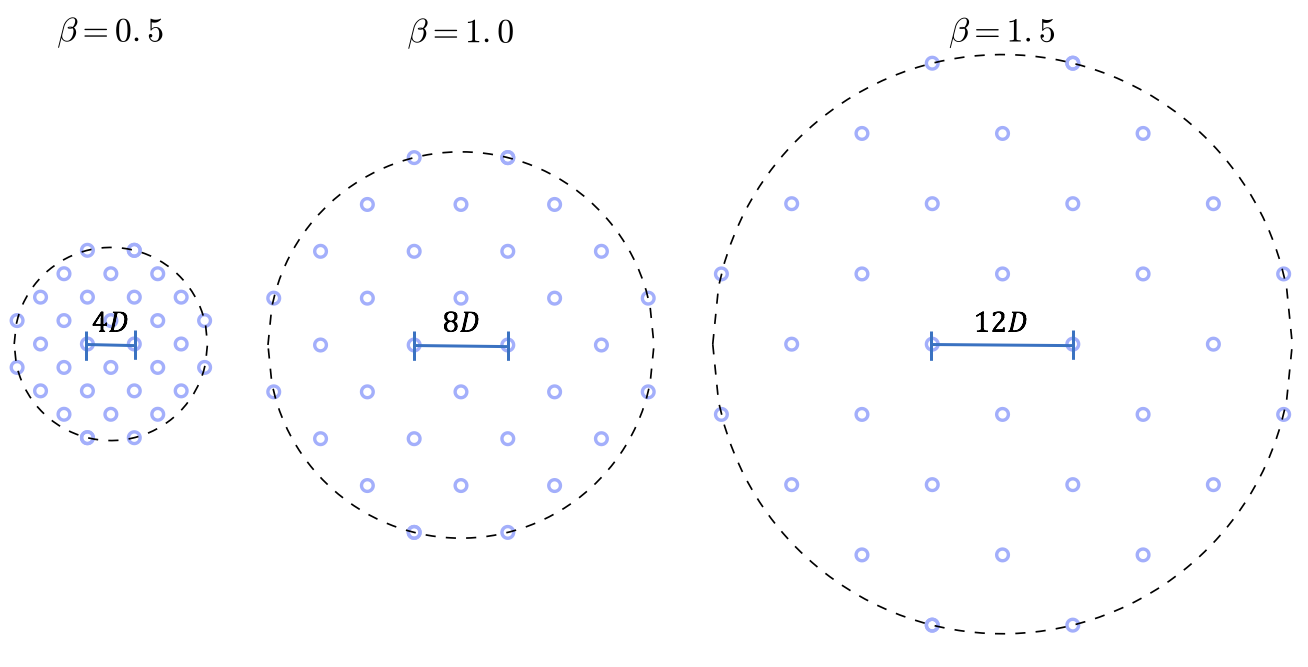
\includegraphics[width=\textwidth]{Figures/circle_spacings.png}
%   \caption{\label{circle_spacings} \textbf{CAPTION HERE}}
% \end{figure}


% \begin{figure}[htbp]
%   \centering
%   \subfloat[]{\includegraphics[trim={0 0 0 0},clip,width=0.33\textwidth]{Figures/amalia0_5.pdf}\label{wp075}}
%   \subfloat[]{\includegraphics[trim={0 0 0 0},clip,width=0.33\textwidth]{Figures/amalia1_0.pdf}\label{wp175}}
%   \subfloat[]{\includegraphics[trim={0 0 0 0},clip,width=0.33\textwidth]{Figures/amalia1_5.pdf}\label{wp275}}
%   \caption{\label{shear_profile}\textbf{CAPTION HERE}}
% \end{figure}